%%%%%%%% ICML 2021 EXAMPLE LATEX SUBMISSION FILE %%%%%%%%%%%%%%%%%

\documentclass{article}

% Recommended, but optional, packages for figures and better typesetting:
\usepackage{microtype}
\usepackage{graphicx}
\usepackage{subfigure}
\usepackage{booktabs} % for professional tables

% hyperref makes hyperlinks in the resulting PDF.
% If your build breaks (sometimes temporarily if a hyperlink spans a page)
% please comment out the following usepackage line and replace
% \usepackage{icml2021} with \usepackage[nohyperref]{icml2021} above.
\usepackage{hyperref}

% Attempt to make hyperref and algorithmic work together better:
\newcommand{\theHalgorithm}{\arabic{algorithm}}

% Use the following line for the initial blind version submitted for review:
% \usepackage{icml2021}

% If accepted, instead use the following line for the camera-ready submission:
\usepackage[accepted]{icml2021}

% The \icmltitle you define below is probably too long as a header.
% Therefore, a short form for the running title is supplied here:
\icmltitlerunning{}

\begin{document}

\twocolumn[
\icmltitle{Data Augmentation as an Inverse Problem}

% It is OKAY to include author information, even for blind
% submissions: the style file will automatically remove it for you
% unless you've provided the [accepted] option to the icml2021
% package.

% List of affiliations: The first argument should be a (short)
% identifier you will use later to specify author affiliations
% Academic affiliations should list Department, University, City, Region, Country
% Industry affiliations should list Company, City, Region, Country

% You can specify symbols, otherwise they are numbered in order.
% Ideally, you should not use this facility. Affiliations will be numbered
% in order of appearance and this is the preferred way.
\icmlsetsymbol{equal}{*}

\begin{icmlauthorlist}
\icmlauthor{Hayden Prairie}{}
\end{icmlauthorlist}

\icmlcorrespondingauthor{Hayden Prairie}{haydenprairie@utexas.edu}

% You may provide any keywords that you
% find helpful for describing your paper; these are used to populate
% the "keywords" metadata in the PDF but will not be shown in the document

\vskip 0.3in
]

% this must go after the closing bracket ] following \twocolumn[ ...

% This command actually creates the footnote in the first column
% listing the affiliations and the copyright notice.
% The command takes one argument, which is text to display at the start of the footnote.
% The \icmlEqualContribution command is standard text for equal contribution.
% Remove it (just {}) if you do not need this facility.

% \printAffiliationsAndNotice{}  % leave blank if no need to mention equal contribution
% \printAffiliationsAndNotice{\icmlEqualContribution} % otherwise use the standard text.

\begin{abstract}
With the growth in the complexity of neural networks and the amount of available compute, the need for larger datasets
has become a bottleneck in the advancements of computer visions. In this paper we explore an new approach to synthetic
data generation by treating data augmentation as an inverse problem. We ultize posterior sampling with latent diffusion
models to in order generate synthetic data through masking. Finally we discuss potential improvements and future work
that can be done. Code is available at \url{https://github.com/Hprairie/Synthetic-ImgGen-PSLD}.
\end{abstract}

\section{Introduction}
\label{introdcution}

In recent years deep learning has made incredible strides in computer vision tasks such as image classification,
object detection, and semantic segmentation. Most advancements within this feild can be attributed to the improvement
of novel architectures, an increase in compute, and access to large datasets. However, the ability to scale a model
without scaling the size of its correspondeing dataset has been show to have diminishing returns \cite{2001.08361}.
The ability to generated large labeled datasets by hand is infeasable and thus the need for unsupervised techniques to create
augmented or synthetic data become's necissary. Niave approaches to data augmentation such as random cropping, flipping,
rotation, etc. have been shown to be effective in some cases, but unfeasable in other cases such as medical imaging, where
niave approaches create unrealistic image domains. More advanced techniques such as generative adversarial networks (GANs)
have been shown to be effictive in creating realistic synthetic data, however these often require large amounts of data in
order to fine tune models.

In the last year the surge in the power of large language models such as GPT-4 has also shown their potential to create synthetic
data. The ability to generate realistic text responses to prompts can be viewed as an inverse problem, where the model is attempting
to find the most likely text given a prompt. A similar approach can be applied to images, where diffusion models can be used to solve
inverse problems and in turn generate synthetic data.

\begin{figure}[ht]
    \vskip 0.2in
    \begin{center}
        \centerline{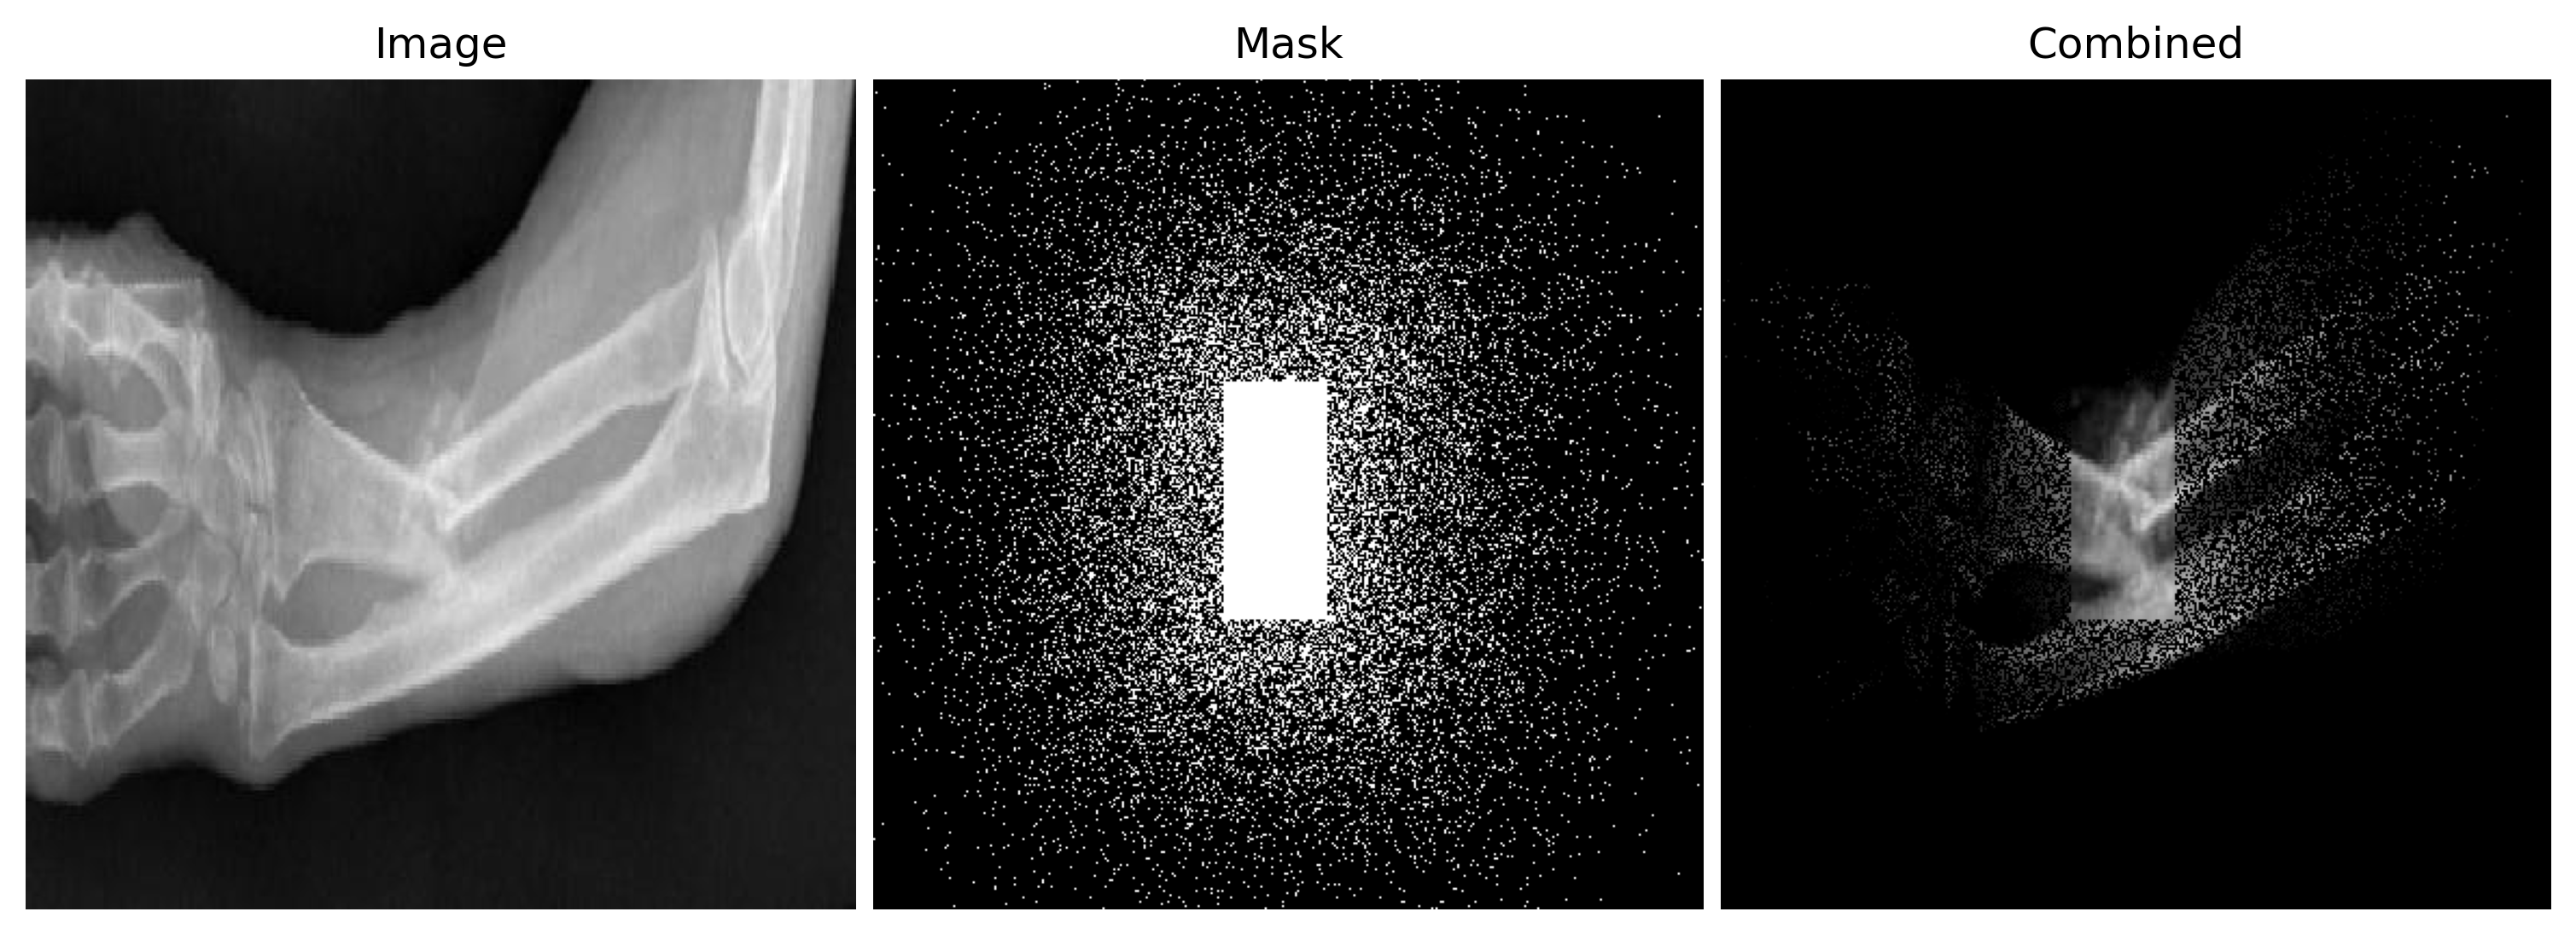
\includegraphics[width=\columnwidth]{Mask.png}}
        \caption{Posterior sampling with latent diffusion (PSLD) is a method of solving linear inverse problems in images by utilizing the power of latent diffusion models such as Stable Diffusion.}
        \label{psld}
    \end{center}
    \vskip -0.3in
\end{figure}

In this paper we explore the use of posterior sampling with latent diffusion models (PSLD) to create synthetic data. PSLD
is a method of solving linear inverse problems in images by utilizing the power of latent diffusion models such as Stable Diffusion. By
generating a mask and then using PSLD to reconstruct the image, variations of the original image can be created,
due mainly the inherent lossy relations of masking pixels. We found these synthetic images to be effective in improving
the performance of object detections models.

The rest of the paper is organized as follows. First we cover the benefits and downsides of niave and advanced data
augmentation techniques. Then we cover our approach of treating augmentation as an inverse problem and utilize diffusion
models for synthetic data generation. Finally we cover the results of our initial expirements and potential improvements along
with future work that can be done.
 

\section{Data Augmentation Techniques}

Data Augementation and synthetic data generation aim to artifically increase the size of training set in order to improve robustness
of computer vision models and prevent overfitting to a training set. Similar to dropout in neural networks, data augmentation can be
useful in leading a model to a more generalizable solution \cite{1708.04896}.

\subsection{Niave Data Augmentation}

Most niave data augmentation techniques apply simple tranformations to the input image while maintaining the label, such as flipping,
cropping, rotating, translation, color jittering, and adding noise. Other more complex techniques such as random erasing aim to occlude
parts of the image allowing the model to learn to focus on other features. These techniques are often effective in improving the performance
of computer vision models to an extent, however they are often ignorant to certain domains such as medical imaging, where simple
transoformations are not applicable to potential real world domains. For example in brain ct scans, linear transformations of the image
would create unrealistic domains that are not representative of test/validation data.

\subsection{Advanced Data Augmentation}

In more recents years the use of GANs have been show to be effective in creating realistic synthitic data. 

\section{Our Approach}

\section{Results}

\section{Discussion and Future Work}

% Acknowledgements should only appear in the accepted version.
\section*{Acknowledgements}

We would like to thank Litu Rout for spending time to help explain his work on solving
inverse problems with PSLD.

% In the unusual situation where you want a paper to appear in the
% references without citing it in the main text, use \nocite
\bibliography{main}
\bibliographystyle{icml2021}

\end{document}


% This document was modified from the file originally made available by
% Pat Langley and Andrea Danyluk for ICML-2K. This version was created
% by Iain Murray in 2018, and modified by Alexandre Bouchard in
% 2019 and 2021. Previous contributors include Dan Roy, Lise Getoor and Tobias
% Scheffer, which was slightly modified from the 2010 version by
% Thorsten Joachims & Johannes Fuernkranz, slightly modified from the
% 2009 version by Kiri Wagstaff and Sam Roweis's 2008 version, which is
% slightly modified from Prasad Tadepalli's 2007 version which is a
% lightly changed version of the previous year's version by Andrew
% Moore, which was in turn edited from those of Kristian Kersting and
% Codrina Lauth. Alex Smola contributed to the algorithmic style files.
